\begin{tikzpicture}
	\savebox\mygraphic{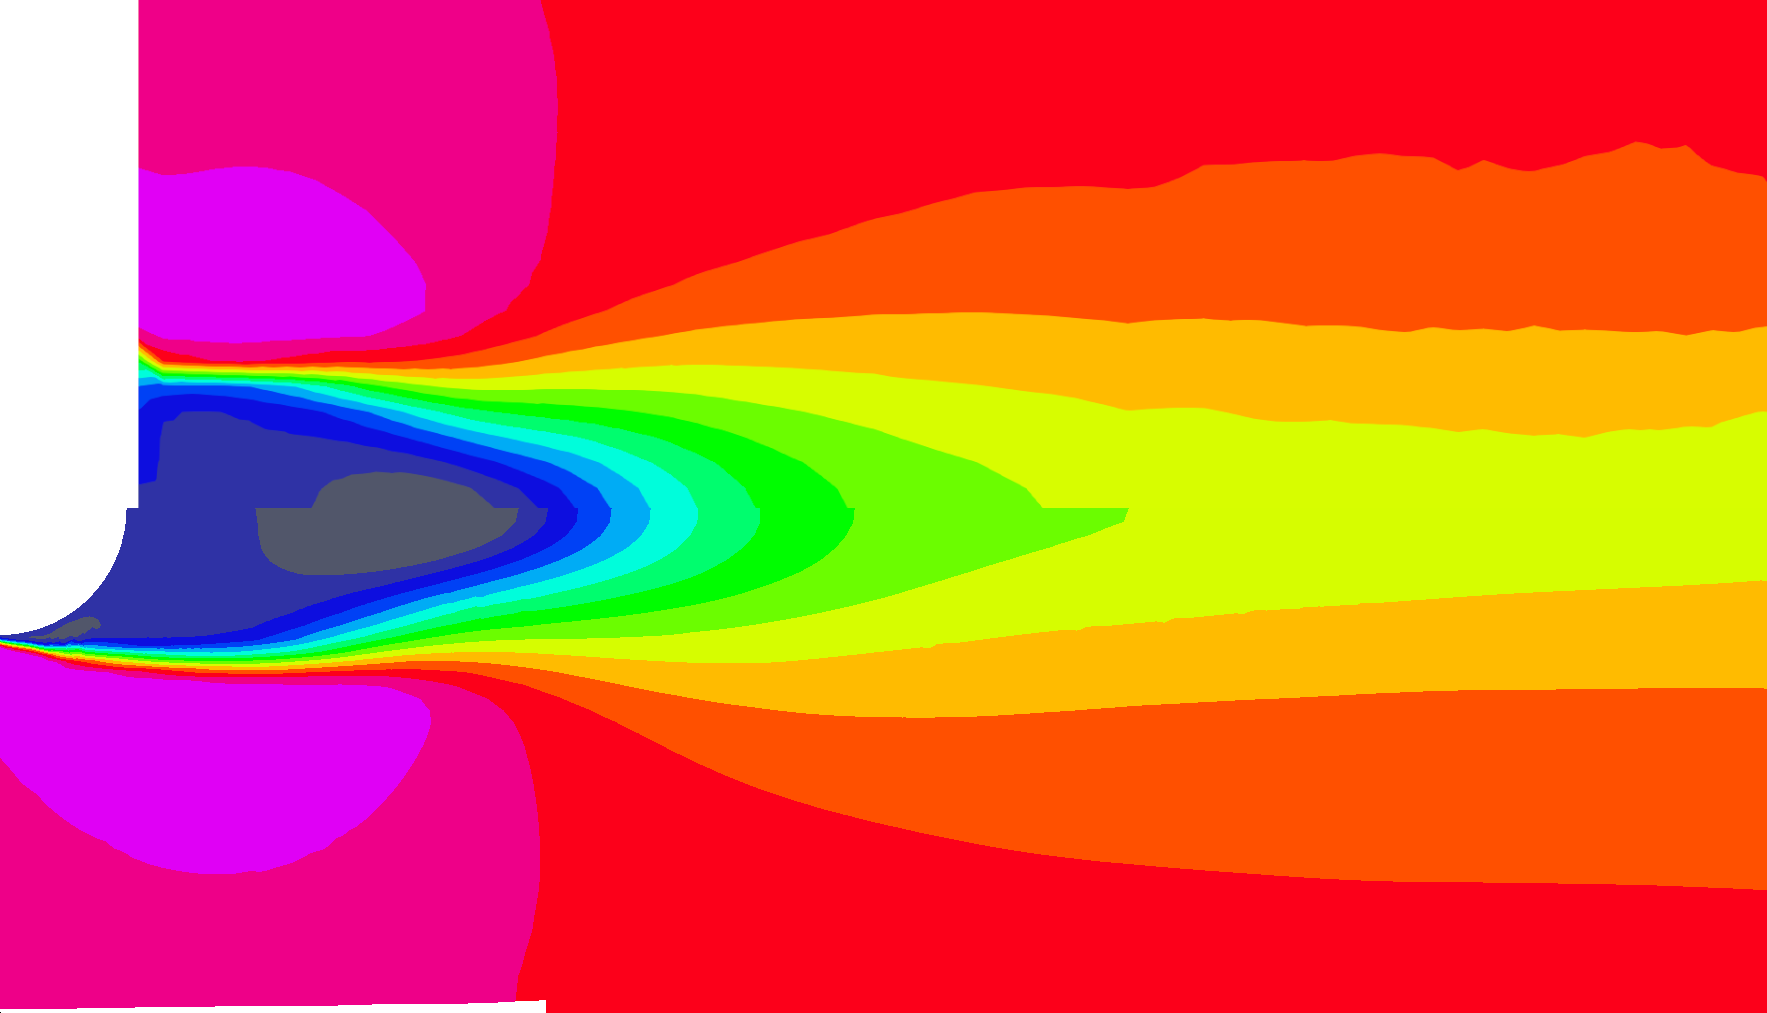
\includegraphics[trim = 0px 0px 0px 0px,clip,width = 0.39\textwidth]{\myImages/res/uXMeanComp.png}}
	\begin{axis}[
		name = plot1,
		xlabel={$x_r$ [--]},
		ylabel={$y_r$ [--]},
		font = \scriptsize,
		xtick distance=1,ytick distance=1,
		width=\wd\mygraphic,
		height=\ht\mygraphic, %height= 5/3*0.5
		enlargelimits=false,
		scale only axis=true,
		tick align=outside,
		x label style = {at={(axis cs:3.5,-2.7)}},
		y label style = {at={(axis cs:-1,0)}},
		ytick pos=left,
		xtick pos=bottom,
		line width = 1.7pt]
		\addplot graphics[xmin=0, xmax=7, ymin=-2, ymax=2,includegraphics={trim = 0px 0px 0px 0px,clip}] {\myImages/res/uXMeanComp.png};
		\fill [white] (axis cs:0.001,-1.997) rectangle (axis cs:0.5,1.997);
		\fill [black!70](axis cs:0,0) circle [radius=0.5];
		\draw [black,dashdotted,line width = 1pt] (axis cs:0,0) -- (axis cs:7,0);
		\node at (axis cs:6.5,1.7) {\scriptsize{PIV}};
		\node at (axis cs:6.5,-1.7) {\scriptsize{CFD}};
		\draw [black!70,dashed,line width = 1pt] (axis cs:3.83,2) -- (axis cs:3.83,-2);
		\node [black!70] at (axis cs:4.1,1.7) {\scriptsize{$\zeta$}};
		\node  at (axis cs:6.7,0.3) {\scriptsize{$\sigma$}};
		\fill [black](axis cs:4,0) circle [radius=0.1];
		\node  at (axis cs:4.2,-0.3) {\scriptsize{$p_{1}$}};
		\fill [black](axis cs:4.53,1.15) circle [radius=0.1];
		\node  at (axis cs:5,1.15) {\scriptsize{$p_{2}$}};
	\end{axis}


	\node [name = osaUx,anchor = south east,at={(plot1.north east)},yshift=0.07cm] {
\includegraphics[width=0.26\textwidth]{\myImages/res/U_x_scale.png}};
	\node [name = ux, anchor = east,at={(osaUx.north west)},yshift=-0.1cm,xshift=-0.1cm] {\scriptsize{$u/u_{\mathrm{in}}$ [--]}};
	\node [name = psi0, anchor = south,at={(osaUx.north)},yshift=-0.2cm,xshift=-1.61cm] {\scriptsize{-0.2}};
	\node [name = psi0, anchor = west,at={(psi0.east)},xshift=0.22cm] {\scriptsize{0.2}};
	\node [name = psi0, anchor = west,at={(psi0.east)},xshift=0.228cm] {\scriptsize{0.6}};
	\node [name = psi0, anchor = west,at={(psi0.east)},xshift=0.228cm] {\scriptsize{1.0}};
	\node [name = psi0, anchor = west,at={(psi0.east)},xshift=0.02cm] {\scriptsize{1.3}};
	% \node [name = psiM05, anchor = north west,at={(osaPsix.south west)},yshift=0.2cm] {\scriptsize{-0.1 \%}};
	% \node [name = psiM05, anchor = north east,at={(osaPsix.south east)},yshift=0.2cm] {\scriptsize{0.1 \%}};

	\savebox\mygraphic{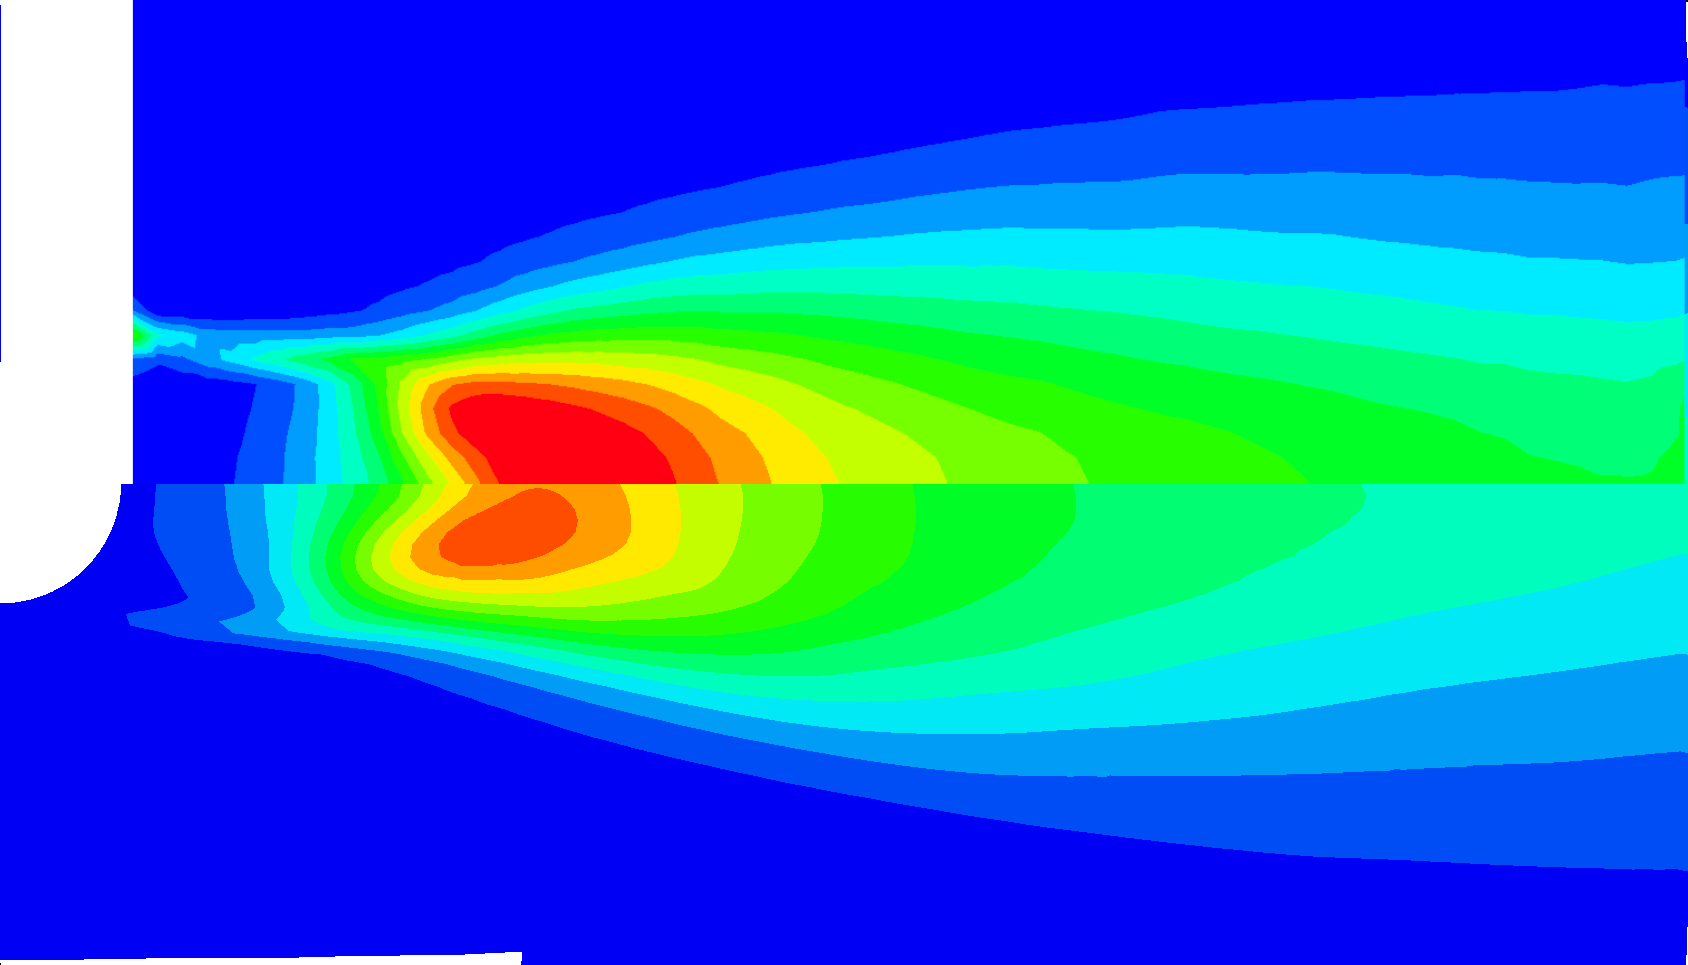
\includegraphics[trim = 0px 0px 0px 0px,clip,width = 0.39\textwidth]{\myImages/res/kMeanComp.png}}
	\begin{axis}[
		name = plot2,
		anchor = west,
		at = {(plot1.east)},
		xshift = 0.4cm,
		xlabel={$x_r$ [--]},
		ylabel={$y_r$ [--]},
		x label style = {at={(axis cs:3.5,-2.7)}},
		y label style = {at={(axis cs:7.8,0)}},
		font = \scriptsize,
		xtick distance=1,ytick distance=1,
		width=\wd\mygraphic,
		height=\ht\mygraphic, %height= 5/3*0.5
		enlargelimits=false,
		scale only axis=true,
		ytick pos=right,
		xtick pos=bottom,
		tick align=outside,
		line width = 1.7pt]
		\addplot graphics[xmin=0, xmax=7, ymin=-2, ymax=2,includegraphics={trim = 0px 0px 0px 0px,clip}] {\myImages/res/kMeanComp.png};
		\fill [white] (axis cs:0.001,-1.997) rectangle (axis cs:0.5,1.997);
		\fill [black!70](axis cs:0,0) circle [radius=0.5];
		\draw [black,dashdotted,line width = 1.0pt] (axis cs:0,0) -- (axis cs:7,0);
		\node  at (axis cs:6.7,0.3) {\scriptsize{$\sigma$}};
		\node [color=white] at (axis cs:6.5,1.7) {\scriptsize{PIV}};
		\node [color=white] at (axis cs:6.5,-1.7) {\scriptsize{CFD}};
	\end{axis}

	\node [name = osak,anchor = south east,at={(plot2.north east)},yshift=0.07cm,xshift=0.1cm] {
\includegraphics[width=0.26\textwidth]{\myImages/res/k_scale.png}};
	\node [name = k, anchor = east,at={(osak.north west)},yshift=-0.1cm,xshift=-0.1cm] {\scriptsize{$k$ [--]}};
	\node [name = psi0, anchor = south,at={(osak.north)},yshift=-0.2cm,xshift=-1.49cm] {\scriptsize{0.00}};
	\node [name = psi0, anchor = west,at={(psi0.east)},xshift=-0.085cm] {\scriptsize{0.06}};
	\node [name = psi0, anchor = west,at={(psi0.east)},xshift=-0.08cm] {\scriptsize{0.12}};
	\node [name = psi0, anchor = west,at={(psi0.east)},xshift=-0.08cm] {\scriptsize{0.18}};
	\node [name = psi0, anchor = west,at={(psi0.east)},xshift=-0.15cm] {\scriptsize{0.24}};
	\node [name = psi0, anchor = west,at={(psi0.east)},xshift=-0.2cm] {\scriptsize{0.28}};
	% \node [name = psi0, anchor = west,at={(psi0.east)},xshift=0.06cm] {\scriptsize{}};
	% \node [name = psi0, anchor = west,at={(psi0.east)},xshift=0.06cm] {\scriptsize{0.6}};
	% \node [name = psi0, anchor = west,at={(psi0.east)},xshift=0.06cm] {\scriptsize{0.6}};
	% \node [name = psi0, anchor = west,at={(psi0.east)},xshift=0.228cm] {\scriptsize{0.6}};
	% \node [name = psi0, anchor = west,at={(psi0.east)},xshift=0.228cm] {\scriptsize{1.0}};
	% \node [name = psi0, anchor = west,at={(psi0.east)},xshift=0.02cm] {\scriptsize{1.3}};
\end{tikzpicture}